\chapter{Documentation du projet}
\section{Analyse du Problème}

Le projet débute par l'analyse du texte expliquant les besoins du client. Notre stratégie consistait à identifier les objets nécessaires pour construire les tables de notre future base de données, en incluant les dépendances fonctionnelles entre eux ainsi que les contraintes de valeurs et de multiplicité.

L'email du refuge a été utilisé pour déterminer tous les attributs de la table \texttt{"refuge"}. De plus, en connaissant l'objet \texttt{"Repas"}, nous avons pu établir une relation permettant de déduire le prix associé à ce repas. L'idée d'avoir une propriété propre a commencé à prendre forme.

Il a été décidé qu'un refuge peut disposer d'au plus un numéro. En ce qui concerne les \texttt{"Formations"}, nous avons observé qu'une formation peut proposer au moins une activité, introduisant ainsi une nouvelle contrainte de multiplicité.

Pour assurer la conformité de notre base de données au Règlement Général sur la Protection des Données (RGPD), nous avons créé un identifiant utilisateur (\texttt{"IdUsr"}) pour préserver les traces de réservations sans avoir besoin de stocker les données clients directement. Ainsi, les données clients sont mieux protégées et peuvent être supprimées si le client en fait la demande.

Afin de bien identifier les réservations pour les refuges et les formations, des identifiants ont été introduits pour jouer le rôle de clés primaires.

















\subsection{Conception du Diagramme Entités/Associations (UML)}

La deuxième étape a été la conception du diagramme Entités/Associations (UML). La table \texttt{"Refuge"} regroupe toutes les informations relatives au refuge. Afin de respecter la contrainte de multiplicité stipulant qu'un refuge peut avoir au plus un numéro, nous avons établi une association sémantique entre la table \texttt{"Refuge"} et la table \texttt{"Ref\_NumTel"}. Une propriété propre relie également \texttt{"Refuge"} à \texttt{"Repas"}, permettant d'indiquer le prix d'un repas dans un refuge spécifique.

La table \texttt{"ReservationRefuge"} est naturellement liée à la table \texttt{"Refuge"} pour indiquer à quel refuge la réservation correspond. Elle est également liée à la table \texttt{"CompteUtilisateur"}, permettant d'identifier à qui appartient cette réservation.

Les données utilisateur sont stockées dans une table distincte du même nom, associée à la table \texttt{"CompteUtilisateur"}, qui ne contient que l'identifiant de l'utilisateur. Cela garantit la conformité au RGPD. De plus, étant donné qu'un utilisateur peut être adhérent ou non, la table \texttt{"Adherents"} est une sous-entité faible de la table \texttt{"Utilisateur"}.

Cette dernière est associée aux tables \texttt{"ReservationFormation"} et \texttt{"LocationMateriel"}. Ces deux tables sont respectivement liées à la table \texttt{"Formations"} par une association sémantique, et à la table \texttt{"LotMateriel"} par une propriété propre déterminant le nombre de pièces réservées et le nombre cassées/perdues.

La table \texttt{"LotMateriel"} est associée à une table texte pour indiquer si un lot peut ou non avoir une description. Elle est également associée à une seule et unique catégorie dans la table \texttt{"Categorie"}. Cette dernière possède une association réflexive permettant de représenter le fait qu'une catégorie mère peut avoir plusieurs sous-catégories ou aucune.

La table \texttt{"Activité"} est associée à \texttt{"Formation"} pour indiquer de quelle formation il s'agit. Elle est également associée à la table \texttt{"LotMateriel"}, indiquant le matériel utilisé pour une certaine activité.


\section{Passage au Relationnel}

Le modèle relationnel de la base de données reflète la structure définie dans le diagramme Entités/Associations (UML) et se traduit en un ensemble de tables interconnectées. Chaque table représente une entité distincte avec ses attributs, les clés primaires et les clés étrangères nécessaires pour maintenir l'intégrité des données.

\begin{enumerate}
     


\item    CompteUtilisateur : La table \textbf{CompteUtilisateur} contient les informations relatives aux utilisateurs, avec un identifiant unique (\texttt{idUsr}). L'entité \textbf{Utilisateur} est associée à cette table, utilisant l'identifiant \texttt{idUsr} comme clé étrangère.

\item    Adherent : L'entité \textbf{Adherent} est représentée par une table du même nom, reliant les utilisateurs adhérents via l'identifiant \texttt{idUsr}, qui agit comme clé primaire et clé étrangère vers \textbf{CompteUtilisateur}.

 \item   Refuge : Les informations sur les refuges sont stockées dans la table \textbf{Refuge}, avec l'email du refuge comme clé primaire. La table \textbf{Propose} associe les repas proposés par chaque refuge avec leurs prix spécifiques.

\item    ReservationRefuge : La réservation d'un refuge par un utilisateur est enregistrée dans la table \textbf{ReservationRefuge}, avec un identifiant unique (\texttt{idResRefuge}). Les liens vers l'utilisateur adhérent et le refuge sont établis via les clés étrangères.

\item    Formation : Les détails des formations sont capturés dans la table \textbf{Formation}, avec l'année et le rang comme clés primaires. La table \textbf{ReservationFormation} enregistre les réservations des formations par les adhérents.

\item    Utilise : L'utilisation du matériel par une activité est modélisée par la table \textbf{Utilise}, reliant les activités aux lots de matériel spécifiques.

\item    LotMateriel : Les caractéristiques des lots de matériel sont enregistrées dans la table \textbf{LotMateriel}, avec une clé primaire composée de la marque, du modèle, et de l'année. La présence d'une date de péremption est facultative.

\item    LocationMateriel : Les locations de matériel effectuées par les adhérents sont enregistrées dans la table \textbf{LocationMateriel}, avec un identifiant unique (\texttt{idLocationMateriel}) et des références aux adhérents.

\item    ReservationPieces : Les réservations spécifiques de pièces de matériel sont gérées par la table \textbf{ReservationPieces}, reliant les réservations aux lots de matériel et aux locations.

\item    DatePeremption : La table \textbf{DatePeremption} stocke les dates de péremption associées aux lots de matériel, liées par la table \textbf{A\_pour\_datePeremption}.
\end{enumerate}

On obtient ainsi le schéma relationnel suivant:\\
\textbf{CompteUtilisateur}( \underline{idUsr} )\\
\textbf{Utilisateur}( \underline{emailUsr}, pwdUsr, nomUsr, prenomUsr, adressUsr, idUsr, sommeDue, sommeRemboursee)\\
\textbf{Adherent}( \underline{idUsr} )\\
\textbf{Refuge}(\underline{email}, nomRefuge, secteurGeo, dateOuverture, dateFermeture, nbPlacesRepas, nbPlacesDormir, texteRepresentatif, typePaiement, prixNuitee)\\
\textbf{RefNumTel}( \underline{numTel}, email)\\
\textbf{ReservationRefuge}( \underline{idResRefuge}, dateResRefuge, heureResRefuge, nbNuitResRefuge, nbRepasResRefuge, prixResRefuge, email, idUsr)\\
\textbf{Repas}( \underline{repas} )\\
\textbf{Propose}( \underline{email}, \underline{repas}, prix)\\
\textbf{Formation}( \underline{annee}, \underline{rang}, nomFormation, dateDemarrage, dureeFormation, nbPlacesFormation, descriptionFormation, prixFormation)\\
\textbf{ReservationFormation}(\underline{idReservationFormation}, rangAttente, annee, rang, idUsr)\\
\textbf{Activite}(\underline{typeActivite})\\
\textbf{A\_pour\_activite}(\underline{anne}, \underline{rang}, \underline{typeActivite}, rang, idUsr)\\
\textbf{LotMateriel}(\underline{marque}, \underline{modele}, \underline{annee}, nbPieces, prix, catgorie)\\
\textbf{Utilise}(\underline{marque}, \underline{modele}, \underline{annee}, \underline{typeActivite})\\
\textbf{Texte}(\underline{texte}, marque, modele, annee)\\
\textbf{Categorie}(\underline{categorie})\\
\textbf{A\_comme\_sous\_categorie}(categorie, \underline{sousCategorie})\\
\textbf{LocationMateriel}(\underline{idLocationMateriel}, dateRecup, dateRetour, idUsr)\\
\textbf{ReservationPieces}(\underline{marque}, \underline{modele}, \underline{annee}, \underline{idLocationMateriel}, nbPiecesReservees, nbPiecesCasseesPerdues)\\
\textbf{DatePeremption}(\underline{datePeremption})\\
\textbf{A\_pour\_date\_peremption}(\underline{marque}, \underline{modele}, \underline{annee}, datePeremption)\\


Chaque table est conçue pour refléter les relations et les contraintes établies lors de la phase de conception, garantissant ainsi une représentation cohérente des données du projet.

\subsection{Formes Normales}
Toutes les tables du schéma relationnel suivent la forme normale de Boyce-Codd-Kent. En effet, il n'y a pas de dépendance non triviale dont la partie gauche n'est pas une clef.
\section{Analyse des Fonctionnalités}

\subsection{Parcours des formations/refuges/matériels disponibles}

\par Cette fonctionnalité permet aux adhérents d'accéder aux informations des lots de matériel disponibles, des formations proposées, ainsi que des refuges disponibles, offrant aux membres une expérience transparente lors de la réservation de matériel, de l'inscription à des formations ou de la planification de séjours en refuge.

\begin{enumerate}

\item \textbf{Lots de Matériel Disponibles}
La méthode `showMaterielCat` permet aux membres du club de visualiser les lots de matériel disponibles. Pour ce faire, la base de données est interrogée pour récupérer des informations telles que le modèle, la marque, l'année, la catégorie, le nombre de pièces disponibles, et la date de péremption des articles. La complexité de cette requête réside dans la gestion des réservations et la vérification de la disponibilité des articles par rapport à leur date de péremption.
 L'objectif est de permettre aux adhérents du club de visualiser les articles disponibles non seulement dans une catégorie spécifique, mais également dans toutes les sous-catégories associées de manière récursive.

\item \textbf{Formations Offertes par le Club}
La deuxième fonctionnalité concerne l'affichage des formations proposées par le club. La méthode `showCourses` récupère les informations essentielles sur les formations, telles que le nom de la formation, le type d'activité associé, la date de démarrage, la durée, et le nombre de places disponibles. Les résultats sont triés de manière à présenter une liste claire et ordonnée pour les adhérents.

\item \textbf{Refuges Disponibles}
Enfin, la troisième fonctionnalité offre aux adhérents la possibilité de visualiser les refuges disponibles. La méthode `showRefuge` permet de trier les refuges par le nom et offre deux options de tri supplémentaires : par dates de début et de fin de gardiennage, ou par le nombre de places disponibles. Cette flexibilité dans l'affichage garantit une meilleure expérience utilisateur, en permettant aux membres de choisir le tri qui correspond le mieux à leurs besoins.
\end{enumerate}

\par L'implémentation de cette base de données offre une solution complète et efficace pour répondre aux besoins des adhérents du club. La conception de requêtes SQL complexes, la gestion des réservations, la vérification des dates de péremption, et la flexibilité dans l'affichage des résultats ont été les principaux défis relevés. Cette fonctionnalité améliore significativement l'expérience des adhérents du club, en leur offrant un accès aux informations essentielles. 


\subsection{Réservation de Refuge}



Ce module offre des fonctionnalités telles que la réservation de refuges, la vérification de l'identité des utilisateurs, et la suggestion de refuges alternatifs en cas d'annulation.



\begin{figure}[H]
    \centering
    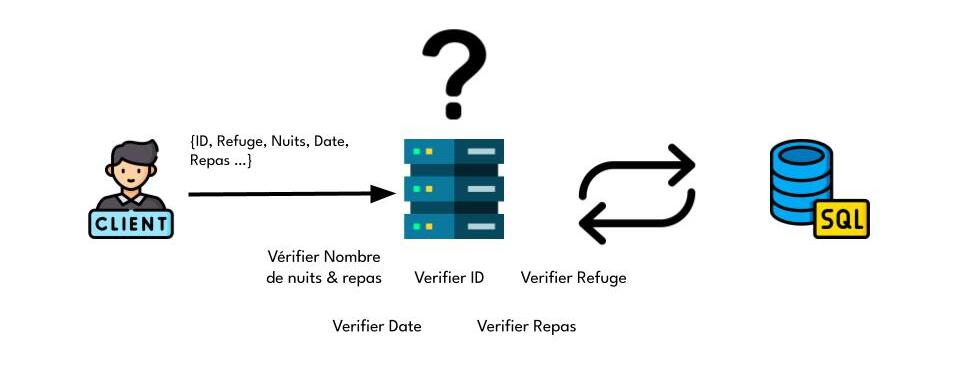
\includegraphics[scale=0.5]{ReserverRefuge.jpg}\\[1cm] 
    \caption{Annulation de réservation}
    \label{fig:enter-label}
\end{figure}



\begin{enumerate}
    
    \item \textbf{Vérification de l'Identité de l'Utilisateur:} Avant d'effectuer une réservation, le programme vérifie l'existence de l'identifiant d'utilisateur (idUsr) dans la table \texttt{CompteUtilisateur}. Cela garantit que seuls les utilisateurs enregistrés peuvent effectuer des réservations.

    \item \textbf{Vérification de l'Existence du Refuge:} Une vérification similaire est effectuée pour s'assurer que le refuge spécifié, identifié par son email, existe dans la table \texttt{Refuge}.

    \item \textbf{Vérification de la Date et des Paramètres:} Le code vérifie la validité de la date de réservation et s'assure que le refuge est ouvert à cette date. De plus, il examine le nombre de nuits et le nombre de repas pour garantir la cohérence des réservations.

    \item \textbf{Calcul du Prix et Insertion dans la Table de Réservation:} Le prix total de la réservation est calculé en interrogeant les tables \texttt{Refuge}, \texttt{Propose}, et \texttt{Repas}. Ensuite, une insertion est effectuée dans la table \texttt{ReservationRefuge}, et le montant dû dans la table \texttt{Utilisateur} est mis à jour.

    \begin{lstlisting}[style=SQL, label=sql-e]
INSERT INTO ReservationRefuge (dateResRefuge, heureResRefuge, nbNuitResRefuge, nbRepasResRefuge, prixResRefuge, email, idUsr) VALUES (?, ?, ?, ?, ?, ?, ?);
UPDATE Utilisateur SET SommeDue = SommeDue + ? WHERE idUSr = ?
    \end{lstlisting}

    \item \textbf{Mise à Jour des Places Disponibles:} Les tables \texttt{Refuge} et \texttt{Propose} sont mises à jour pour refléter les nouvelles réservations et les places disponibles.

    \item \textbf{Annulation de Réservation avec Suggestion de Refuges Alternatifs:} Lorsqu'une annulation de réservation est initiée, le programme vérifie d'abord l'existence de la réservation dans la table \texttt{ReservationRefuge}. En cas de succès, la réservation est supprimée, et des refuges alternatifs du même secteur géographique sont suggérés.
    
\end{enumerate}
 

\begin{figure}[H]
    \centering
    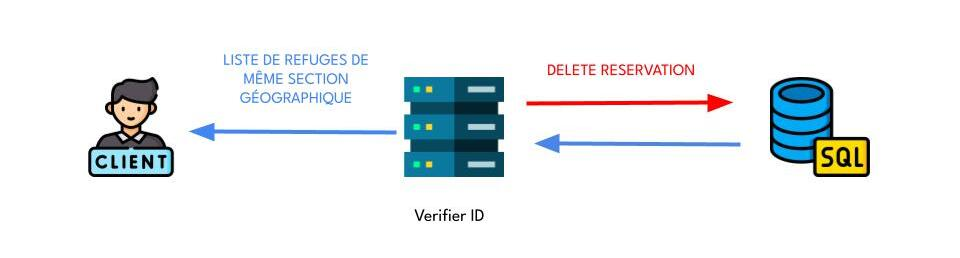
\includegraphics[scale=0.5]{AnnulerReservation.jpg}\\[1cm]
    \caption{Garantir l'intégrité des données}
    \label{fig:enter-label}
\end{figure}




\subsection{Réservation de Formation}
Pour la réservation d'une formation (et éventuelement l'annulation d'une réservation), il faut que l'utilisateur fournisse l'année et le rang qui identifient la formation (ou bien l'idReservationFormation pour l'annuler). Puis la fonctionnalité se réalise en suivant plusieurs étapes:
\begin{enumerate}
    \item \textbf{L’analyse des réservations qui existent déjà:}\\
Cette étape est nécessaire pour savoir l'état de la formation que l'on veut réserver: si elle est pleine ou pas. Ainsi, il faut calculer le nombre de réservations déja effectués, en utilisant la requête : 
    \begin{lstlisting}[style=SQL, label=sql-e]
SELECT COUNT(*) FROM ReservationFormation WHERE annee = ? AND rang = ? AND rangAttente = 0;
\end{lstlisting}
Puis, on compare ce résultat avec le nombre de places que la formation offre. Et si, la formation est déjà pleine, la réservation sera mise en liste d'attente et son rang sera calculé par la requête :
\begin{lstlisting}[style=SQL, label=sql-e]
 SELECT * FROM ReservationFormation WHERE annee = ? AND rang = ? AND rangAttente >= 1;
    \end{lstlisting}

    \item \textbf{L’insertion de la réservation:}\\
En tenant compte de l'analyse qu'on vient de faire, on doit passer à l'insertion de la réservation dans notre base de données. Mais un problème s'est posé lors de notre 1ère approche. Puisqu'on doit renvoyer à l'utilisateur l'id de sa réservation pour qu'il puisse l'annuler après s'il veut. En mettant en place une séquence qui génère automatiquement les identifiants, il sera difficile de connaître l'id qui a été utilisé (un utilisateur peut réserver la même formation plusieurs fois...). Ainsi, on choisit les identifiants manuellement, en utilisant les requêtes suivantes: 
\begin{lstlisting}[style=SQL, label=sql-e]
SELECT MAX(idReservationFormation) FROM ReservationFormation;
INSERT INTO ReservationFormation(idReservationFormation, rangAttente, annee,rang, idUsr) VALUES (?, ?, ?, ?, ?);
\end{lstlisting}
Avec (dans le cas où la réservation est mise dans la liste d'attente): rangAttente = taille de la hashMap où on stocke les réservations en liste d'attente + 1. (On  va plus détailler sur le choix de la hashMap dans la partie qui suit car elle n'est réellement utilisée que dans le cas d'une annulation)

    \item \textbf{L’annulation d’une réservation:}\\
Dans le cas où l'utilisateur souhaite annuler sa réservation, on crée une HashMap qui contient les réservations qui sont aussi en liste d'attente mais qui ont un rangAttente supérieur à celui de la réservation qu'on veut annuler (clé = idReservationFormation et valeur = rangAttente), car c'est eux qui seront touchées par cette annulation. Puis, on supprime la réservation de la base de données par : 
\begin{lstlisting}[style=SQL, label=sql-e]
DELETE FROM ReservationFormation WHERE idReservationFormation = ?;
\end{lstlisting}
Et pour chaque réservation dans la hashMap, on decrémente son rangAttente par 1 en utilisant la requête :
\begin{lstlisting}[style=SQL, label=sql-e]
UPDATE ReservationFormation SET rangAttente = rangAttente - 1 WHERE idReservationFormation = ?;
\end{lstlisting}

Pour chacune de ces réservations, on insère dans un tableau Message de notre base de données un message qui signale le développement de la situation de leur réservation (Passage en liste principale par exemple). Et chaque utilisateur pourra lire ses messages lorsqu'il le souhaite comme une sorte de boîte mail.
\end{enumerate}


\subsection{Location et Retour de Matériel}
La location et le retour du matériel sont des étapes clés du cahier des charges, et nous nous sommes efforcés de respecter les souhaits du client.

Pour la location de matériel, l'utilisateur est requis de nous fournir le ou les lots qu'il souhaite réserver. En effet, l'utilisateur a la possibilité de louer plusieurs lots au sein d'une même réservation.

 Chaque réservation est identifiée par un numéro unique, idLocationMateriel, propriété que nous avons ajoutée dans la table LocationMateriel pour faciliter la traçabilité de chaque transaction, y compris le retour du matériel.


Chaque lot de matériel est identifié par la marque, le modèle et l'année.  L'utilisateur nous transmet ces informations, ainsi que le nombre d'unités qu'il souhaite louer, accompagné des dates de récupération et de retour de location.  

Une fois ces détails reçus, nous procédons à plusieurs vérifications pour garantir que la location puisse être effectuée. Ces vérifications englobent divers critères.

\begin{enumerate}
    \item \textbf{La vérification de la disponibilité du matériel}\\
    Pour évaluer la disponibilité des lots demandés par l'utilisateur, nous examinons les réservations existantes ainsi que le nombre total d'unités disponibles. En cas d'insuffisance d'unités, un message est immédiatement affiché à l'utilisateur, l'informant de la contrainte.
    Ceci grâce à la requête sql suivante (Les "?" remplaçant les informations fournies): \\
    \\
    \begin{lstlisting}[style=SQL, label=sql-e]
SELECT lm.modele,lm.marque,lm.annee,(lm.nbPieces - rp.nbPiecesReservees - rp.nbPiecesCasseesPerdues)
FROM ReservationPieces rp
JOIN  LotMateriel lm 
ON rp.marque = lm.marque and rp.modele = lm.modele and rp.annee = lm.annee
JOIN LocationMateriel locm
ON rp.idLocationMateriel = locm.idLocationMateriel
WHERE locm.dateRetour >= ? and locm.dateRecup <= ?
UNION
SELECT lm.modele,lm.marque,lm.annee,lm.nbPieces
FROM LotMateriel lm 
WHERE (lm.modele, lm.marque, lm.annee) NOT IN
(SELECT rp.modele, rp.marque, rp.annee FROM ReservationPieces rp)
    \end{lstlisting}
    La première section de cette requête examine la disponibilité en fonction des locations déjà effectuées. La deuxième section vise à s'assurer que l'utilisateur ne demande pas plus d'unités que celles disponibles en stock initial.
    \item \textbf{La vérification de la durée de la location}\\
    Tout d'abord, nous veillons à ce que l'utilisateur fournisse des dates valides, impliquant une date de récupération postérieure à la date actuelle et une date de retour postérieure à la date de récupération. Cette étape garantit l'intégrité chronologique du processus de location.
    
    En parallèle, nous effectuons une vérification pour nous assurer que la durée de la location n'excède pas deux semaines. Cette limitation vise à répondre aux paramètres définis pour une gestion optimale des réservations. En cas de non-conformité à ces critères, des messages d'erreur sont générés pour guider l'utilisateur dans la soumission de dates adéquates.
\end{enumerate}
Une fois que toutes les vérifications ont été effectuées et que tout est conforme, la location est confirmée. Au moyen d'une requête sql "INSERT INTO", les informations correspondantes sont ajoutées à la table LocationMateriel, ainsi qu'à la table ReservationsPieces pour assurer une gestion complète des réservations, y compris les détails spécifiques des pièces réservées.

En ce qui concerne le retour de matériel, nous partons du principe que l'utilisateur effectue le retour dans les délais convenus. Il doit nous fournir les détails du lot qu'il souhaite retourner, ainsi que le nombre éventuel de pièces abîmées/perdues. En cas de pièces cassées, le cahier des charges nous oblige à les retirer du lot. Toutefois, pour assurer la traçabilité, ces pièces sont conservées dans le total du lot, c'est-à-dire dans la table LotMateriel, mais elles sont exclues du nombre de pièces disponibles pour les futures réservations.

Par ailleurs, nous effectuons le calcul du coût des pièces endommagées, que nous ajoutons à la somme due par l'utilisateur dans la table Utilisateur. Cette approche garantit une gestion précise des retours, en tenant compte des dommages éventuels et de leur impact sur la facturation globale de l'utilisateur.


\section{Droit d'oubli}

Dans le cadre de la mise en œuvre du droit à l'oubli au sein de notre système de gestion, nous avons développé un processus en huit étapes visant à garantir la suppression complète des données d'un utilisateur tout en préservant l'intégrité des relations au sein de la base de données.

La première étape consiste à supprimer toutes les données liées à l'utilisateur, assurant ainsi une élimination exhaustive des informations sensibles. Par la suite, nous générons un nouveau ID utilisateur, l'ajoutons à la table CompteUtilisateur, ainsi qu'à la table EstAdherent, permettant ainsi une reconstruction sécurisée de l'identité de l'utilisateur dans ces contextes.

Les étapes suivantes impliquent la modification des ID utilisateur dans les tables RéservationRefuge, ReservationFormation et LocationMatériel, afin de refléter le nouveau lien avec le compte utilisateur généré. Cette démarche garantit la cohérence des références croisées au sein de notre base de données.

La septième étape vise à éliminer toute trace de l'ancien ID de l'utilisateur de la table EstAdherent, assurant ainsi une dissociation complète avec les adhérences précédentes. Enfin, dans la huitième étape, nous supprimons définitivement l'ancien ID utilisateur de la table CompteUtilisateur, concluant ainsi le processus du droit à l'oubli.

Ce processus rigoureux assure la conformité avec les réglementations de protection des données en vigueur, garantissant la confidentialité et la sécurité des informations personnelles tout en respectant le droit de chaque utilisateur à l'oubli.

\section{Guide d'emploi de l'interface textuelle}




